\documentclass{article}
\usepackage{setspace}
\usepackage{booktabs}
\usepackage{titlesec}
\usepackage{subcaption}
\usepackage[T1]{fontenc}
\usepackage{enumitem}
\usepackage{cite}
\usepackage{hyperref}
\usepackage{minted}
\usepackage{caption}
\usepackage{indentfirst}
\usepackage{subcaption}
\usepackage{enumitem}
\usepackage{appendix}
\usepackage{graphicx}

\usepackage[letterpaper,top=2cm,bottom=2cm,left=3cm,right=3cm,marginparwidth=1.75cm]{geometry}

\begin{document}
\onehalfspacing
\begin{titlepage}
   \begin{center}
       \vspace*{7cm}
    \huge
       \textbf{Big Data Analytics - Milestone 1 report}
       \vspace{0.5 cm}
       \huge
       
       Real-time prediction of Wikipedia edit dynamics based on global news events       
       \vspace{1.5 cm}
    \large
    
       \textbf{Team: Byte Me Analytics}
       \vfill
    \large
       \vspace{0.7 cm}
    
       University Name: Warsaw University of Technology\\
       Department Name: Faculty of Mathematics and Information Science\\ 
       Date: 20th of October, 2025\\
            
   \end{center}
\end{titlepage}


\begin{titlepage}
   \begin{center}
       \vspace*{0.7 cm}
    \tableofcontents        
   \end{center}
\end{titlepage}


\section{High-level project description}
\subsection{Project overview}
Our project depends on building a Big Data system to predict in real-time the intensity of editing on English-language Wikipedia pages. The system will analyze the general correlation between the characteristics of global news events (such as their volume and sentiment from the GDELT stream) and the overall intensity of the Wikipedia changes stream.
\\
As a crucial analytical element as well as the major project's challenge, the system will undergo an attempt of a dynamic entity-level mapping. We will try to identify specific entities in GDELT data, for instance people, organizations, locations etc. and link them to edits on their corresponding Wikipedia pages.
\\
Moreover, using machine learning, the system will generate predictions which may serve as early warnings of so called ``edit wars''\footnote{\href{https://en.wikipedia.org/wiki/List_of_edit_wars_on_Wikipedia}{List of edit wars on Wikipedia}}. The key components of the project will consist of an interactive dashboard, trained prediction model and automated Big Data architecture.  


\subsection{Business process diagram}

Figure~\ref{fig:busineess} illustrates the main workflow of the system from the perspective of a typical user or analyst interacting with the dashboard and the backend system.

\begin{figure}[!h]
    \centering
    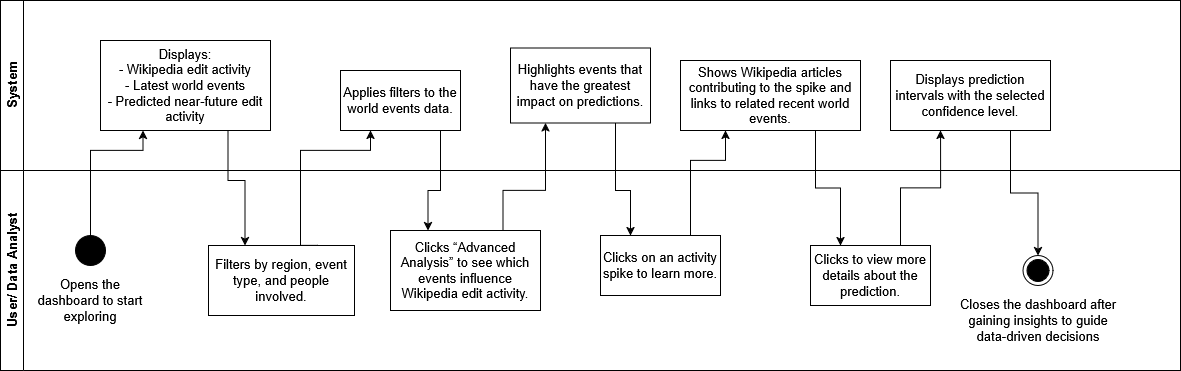
\includegraphics[width=1\linewidth]{business_process.png}
    \caption{Business process diagram}
    \label{fig:busineess}
\end{figure}

The sequence begins with the User opening the dashboard, prompting the System to display three main elements: Wikipedia edit activity, the latest world events, and predicted near-future edit activity. The User can filter the data by region, event type, and people involved. The System updates the displayed world events data according to the applied filters.

For deeper insights, the User clicks “Advanced Analysis,” leading the System to highlight events that most strongly influence Wikipedia edit predictions. When the User selects a specific activity spike, the System reveals the contributing Wikipedia articles and links them to related recent world events. Further exploration allows the User to view detailed prediction data, with the System showing prediction intervals at the chosen confidence level. The sequence concludes with the User closing the dashboard after obtaining actionable, data-driven insights.

\section{Preliminary investigation of data sources}

For this project, two independent, publicly available and highly dynamic data sources will be used. A combination of them allows the application of stream processing techniques. 


\subsection{Source 1: Wikipedia Recent Changes Stream}

The first source of choice is an open, real-time data stream provided by the \textit{Wikimedia Foundation}. The service is implemented as a \textit{Server-Sent Events (SSE)} stream, accessible through HTTP using chunked transfer encoding\footnote{\href{https://wikitech.wikimedia.org/wiki/Event_Platform/EventStreams_HTTP_Service}{Wikimedia Event Platform – EventStreams HTTP Service, Wikimedia Foundation}}.


Each message in the stream represents an individual edit or change in one of the Wikimedia projects. The data are sent in JSON file format, and are compliant with the schema defined by the Wikimedia event system, for instance \texttt{recentchange} stream. A typical record consists of the following attributes: 
\begin{itemize}
    \item \textbf{Metadata:} a unique event ID, timestamp and wiki ID, for instance \texttt{enwiki}. 
    \item \textbf{Edit information:} user name or IP address, page title, version ID, edit comment and flags such as \texttt{minor}, \texttt{new}, \texttt{bot} etc.\footnote{\href{https://schema.wikimedia.org/repositories/primary/jsonschema/mediawiki/recentchange/1.0.0.yaml}{Data schema \texttt{recentchange} – Wikimedia Schema Repository}};
    \item \textbf{Change metrics:} a difference in number of bytes - change size, namespace as well as page length after editing.
\end{itemize}

Moreover, stream is highly dynamic and works in continuous manner. From Wikimedia data it turns out that that across all projects, the average number of edits exceeds 3 edits per second\footnote{\href{https://meta.wikimedia.org/wiki/Wikimedia_in_figures/Wikipedia}{Wikimedia in figures – Wikipedia, Meta-Wikimedia}}. On the other hand, on the English-language Wikipedia itself, based on the monthly statistics, an average number of edits correpsonds to about 5 edits per second\footnote{\href{https://en.wikipedia.org/wiki/Wikipedia}{Wikipedia – Overview and statistics, English Wikipedia}}. What is interesting, during moments of heightened interest in a given topic, for instance during media events, significantly greater changes can be observed - even tens or hundreds of edits per second. However, it is important to emphasize that this is an estimate, not a guaranteed, fixed value.

\paragraph{}
To sum up, the characteristic of the data is as follows:
\begin{itemize}
\item \textbf{Type:} event-based data in JSON format (semi-structured). 
\item \textbf{Volume:} averages around 3-5 events per second across the Wikimedia. Local peaks for given pages or topics can be higher.
\item \textbf{Velocity:} continuous, real-time data streaming.
\end{itemize}


\subsection{Source 2: The GDELT Event Database}
The GDELT (Gloabl Database of Events, Language and Tone) database, supported by the Google Jigsaw, monitors the world's brodcast, print, and web news from nearly every corner of ever country in over 100 languages and identifies the people, locations, organizations, themes, events and other occurrences driving our global society every single day\footnote{\href{https://www.gdeltproject.org/}{The GDELT Project}}. Besides, the entire GDELT database is free and the raw data files can be downloaded and analyzed using \textit{GDELT Analysis Service} or at a limitless scale with \textit{Google BigQuery}.


Users can download the entire underlying event and graph datasets in CSV format. Depending on the complexity of use cases, different GDELT databases can be utilized. The ones that we will use in our project are \textit{GDELT 2.0 Event Database} an well as \textit{GDELT 2.0 Global Knowledge Graph (GKG)}\footnote{\href{https://www.gdeltproject.org/data.html\#rawdatafiles}{The GDELT Project - Raw Data Files}}. 


\subsubsection{GDELT 2.0 Event Database}
It comprises of  a quarter-billion records organized into a set of tab-delimited files ordered by date. Yet, they are named with a \texttt{.CSV} extension in order to address some software packages which would not accept \texttt{.TXT} or \texttt{.TSV} files. 

Furthermore, comparing to \textit{GDELT 1.0}, it offers new features. The most significant one is that the data updates every 15 minutes. It also includes events reported in articles published in the 65 live translated languages. The core event table is fairly the same with a few extra columns, but there is a new ``mentions'' table. Lastly, the newer version introduces the measurements of more than 2300 emotions and themes from every article, as well as a massive inventory of the media of the non-Western world. More of the advancements can be found in \textit{GDELT 2.0 Global Knowledge Graph Codebook (V2.1)} section\footnote{\href{https://blog.gdeltproject.org/gdelt-2-0-our-global-world-in-realtime/}{GDELT 2.0: Our Global World in Realtime}}.   

Based on the informations from the Codebook, a ``typical'' record consists of the following field groups:

\begin{itemize}
    \item \textbf{V2.1DATE}: it is an article publication date in the format \texttt{YYYYMMDDHHMMSS} (a timestamp). 
    \item \textbf{V1PERSONS}: list of all recognized people in the article.
    \item \textbf{V1ORGANIZATIONS}: list of all recognized organizations (companies, government agencies, NGOs, etc.).
    \item \textbf{V1LOCATIONS}: list of all recognized locations (cities, countries, regions).
    \item \textbf{V1.5TONE}: A block containing six key emontional dimensions for the entire article: \texttt{Tone}, \texttt{Positive Score}, \texttt{Negative Score}, \texttt{Polarity}, \texttt{Activity Reference Density}, 
    \texttt{Self/Group Reference Density} and \texttt{Self/Group Reference Density}. 
\end{itemize}


\subsubsection{GDELT 2.0 Global Knowledge Graph (GKG)}

\textit{GDELT 2.0 Global Knowledge Graph (GKG)} is a significantly expanded, near-real-time version of its predecessor (GDELT 1.0). Like version 1.0, GKG aims to connect all people, organizations, locations, emotions, topics, counts, events, and sources into a single global network. 
Similarly to the previously described \textit{GDELT 2.0 Event Database}, the key enhancements for GDELT 2.0 that are fundamental to our project are multilingual processing and translation of articles from 65 languages as well as a high frequency of updates - each per 15 minutes. 

\paragraph{}
Therefore, the characteristic of both the \textit{GDELT 2.0 Event Database} and \textit{GDELT 2.0 Global Knowledge Graph (GKG)} can be summarized as follows:

\begin{itemize}
\item \textbf{Type:} structured data, delivered as CSV, tab-delimited files. Each record represents a single article and contains a rich set of fields. Key to our project are fields identifying entities such as V1PERSONS, V1ORGANIZATIONS, V1LOCATIONS) and the V1.5TONE. 
\item \textbf{Volume:} very high. The system processes global media in 65 languages, generating millions of records daily and hundreds of megabytes of data in every 15-minute interval. 
\item \textbf{Velocity:} near real-time. According to the documentation, new data files are published every 15 minutes which allows for data aggregation in short time periods. 
\end{itemize}



\section{Data processing assumptions}
\subsection{High-level data flow diagram}

Figure~\ref{fig:data_flow} presents the high-level data flow of the proposed system, describing how information moves from external sources to the final user dashboard.

\begin{figure}[h]
    \centering
    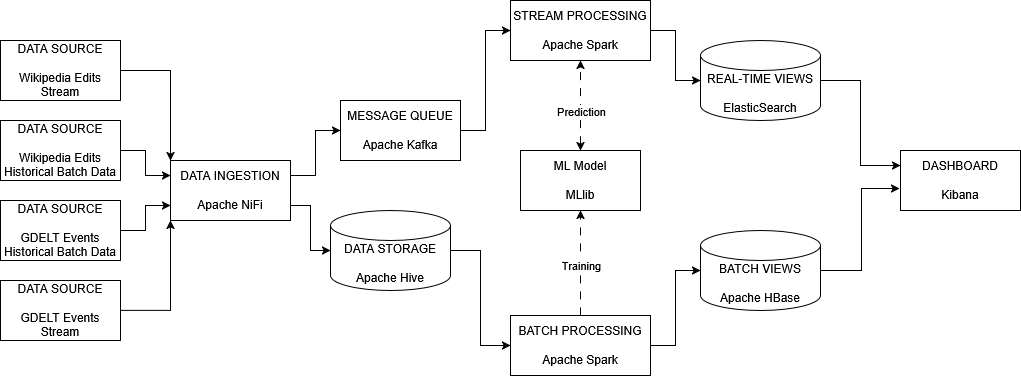
\includegraphics[width=0.9\linewidth]{data_flow.png}
    \caption{High-level data flow diagram}
    \label{fig:data_flow}
\end{figure}

The process begins with two main data sources:
\begin{itemize}
    \item Wikipedia Edits, which provide real-time information on changes made to Wikipedia pages
    \item GDELT Events, representing global media coverage and event metadata.
\end{itemize}
Both data streams are first handled by the data ingestion layer, implemented using Apache NiFi.
The ingested data are then sent to two parallel destinations:
Apache Kafka as a message queue for real-time streaming and
Apache Hive as data storage for batch processing and historical analysis.
For real-time processing, Apache Spark Streaming consumes data from Kafka and uses the trained MLlib model to perform live predictions on editing activity. The resulting predictions are stored in Elasticsearch, forming the real-time views.
Simultaneously, batch processing is performed in Apache Spark, using data stored in Hive to periodically train and update the machine learning model. The outcomes of batch computations are stored in Apache HBase, forming the batch views.
Finally, both real-time and batch views are accessed by the Kibana dashboard, which visualizes trends, correlations, and predictive insights for analysts. This design enables continuous analysis, combining real-time monitoring with historical context.


\section{Proposed solution infrastructure}
\subsection{Technology stack overview}

\paragraph{Data ingestion: Apache NiFI}
Automates data retrieval from the Wikipedia Recent Changes and GDELT feeds. Provides flow control, scheduling, and data source before routing to storage or messaging layers. 

\paragraph{Message queuing: Apache Kafka}
Serves as a high-throughput buffer decoupling data ingestion and processing. Each data stream is assigned to a dedicated topic for reliable delivery and replay 

\paragraph{Data processing: Apache Spark}
Performs large-scale computation in both batch and streaming modes. Spark Streaming handles real-time analytics, while Spark SQL and MLlib manage batch aggregation and machine learning.

\paragraph{Data storage: Hadoop ecosystem}
Apache Hadoop (HDFS) provides distributed storage for raw and processed data, while Apache Hive serves as a data warehouse enabling SQL-style access for analysis and model training. 

\paragraph{Visualisation and search: Elasticsearch \& Kibana}
Elasticsearch stores aggregated metrics and prediction results for fast querying. Kibana provides an interactive dashboard visualising editing intensity, event trends, and sentiment patterns. 

\paragraph{Deployment and version control}
All services are containerized with Docker for consistent deployment. Source code and workflow definitions are managed in GitHub, ensuring collaboration and reproducibility


\subsection{Main architecture components}

The system follows a Lambda Architecture model combining batch and real-time processing.

\paragraph{1. Data ingestion}
NiFi collects, transforms, and standardizes records from Wikipedia and GDELT using dedicated data transformation flows. It then publishes live data to Kafka and also writes to HDFS to store historical data for later analysis.

\paragraph{2. Messaging}
Kafka buffers incoming events and enables scalable, fault-tolerant communication between NiFi
and Spark. Topics are structured by data source and event type.

\paragraph{3. Stream processing layer}
Spark Streaming consumes data from Kafka, performs aggregation, and applies pre-trained
MLlib models to predict Wikipedia edit intensity in near real time. Results are written to
Elasticsearch.

\paragraph{4. Batch processing and storage layer}
Spark SQL processes historical data stored in Hive to compute long-term correlations and retrain machine-learning models, which are then deployed to the streaming layer. It also prepares aggregated datasets for batch visualizations, enabling analysts to explore historical trends and patterns. HDFS stores all raw and aggregated datasets, while Hive organizes them for structured queries.

\paragraph{5. Serving layer}
Elasticsearch stores views generated from streaming processes, enabling near real-time analytics. HBase maintains views of historical datasets prepared by the batch processing layer for efficient batch queries and analysis.

\paragraph{6. Visualization}
Kibana provides interactive dashboards for analysts to explore event and editing patterns, using data stored in both Elasticsearch and HBase.

\paragraph{7. Deployment and orchestration}
All components are deployed as Docker containers managed with Docker Compose. This ensures
modular setup, easy maintenance, and reproducibility of the full analytics pipeline.


\section{Team members and tasks allocation}

The initial task allocation prior to the next milestone is presented in Table~\ref{tab:task_allocation}.

\begin{table}[h!]
\centering
\begin{tabular}{| p{4.5cm} | p{7.5cm} |}
\hline
\textbf{Name and Surname} & \textbf{Tasks} \\
\hline
Alicja Charuza &
    \begin{itemize}[nosep, leftmargin=1.5em]
        \item Wikipedia data acquisition module \& tests
    \end{itemize} \\
\hline

Hubert Jaczyński &
    \begin{itemize}[nosep, leftmargin=1.5em]
        \item GDELT data acquisition module \& tests
    \end{itemize} \\
\hline


Aleksandra Kłos &
    \begin{itemize}[nosep, leftmargin=1.5em]
        \item GDELT data preprocessing module \& tests
    \end{itemize} \\
\hline

Martyna Kuśmierz &
    
    \begin{itemize}[nosep, leftmargin=1.5em]
        \item Wikipedia data preprocessing module \& tests
    \end{itemize} \\
\hline
\end{tabular}
\caption{Task allocation for the project team.}
\label{tab:task_allocation}
\end{table}



\end{document}



